\section{Hardware}
\begin{figure}[H]
	\centering
	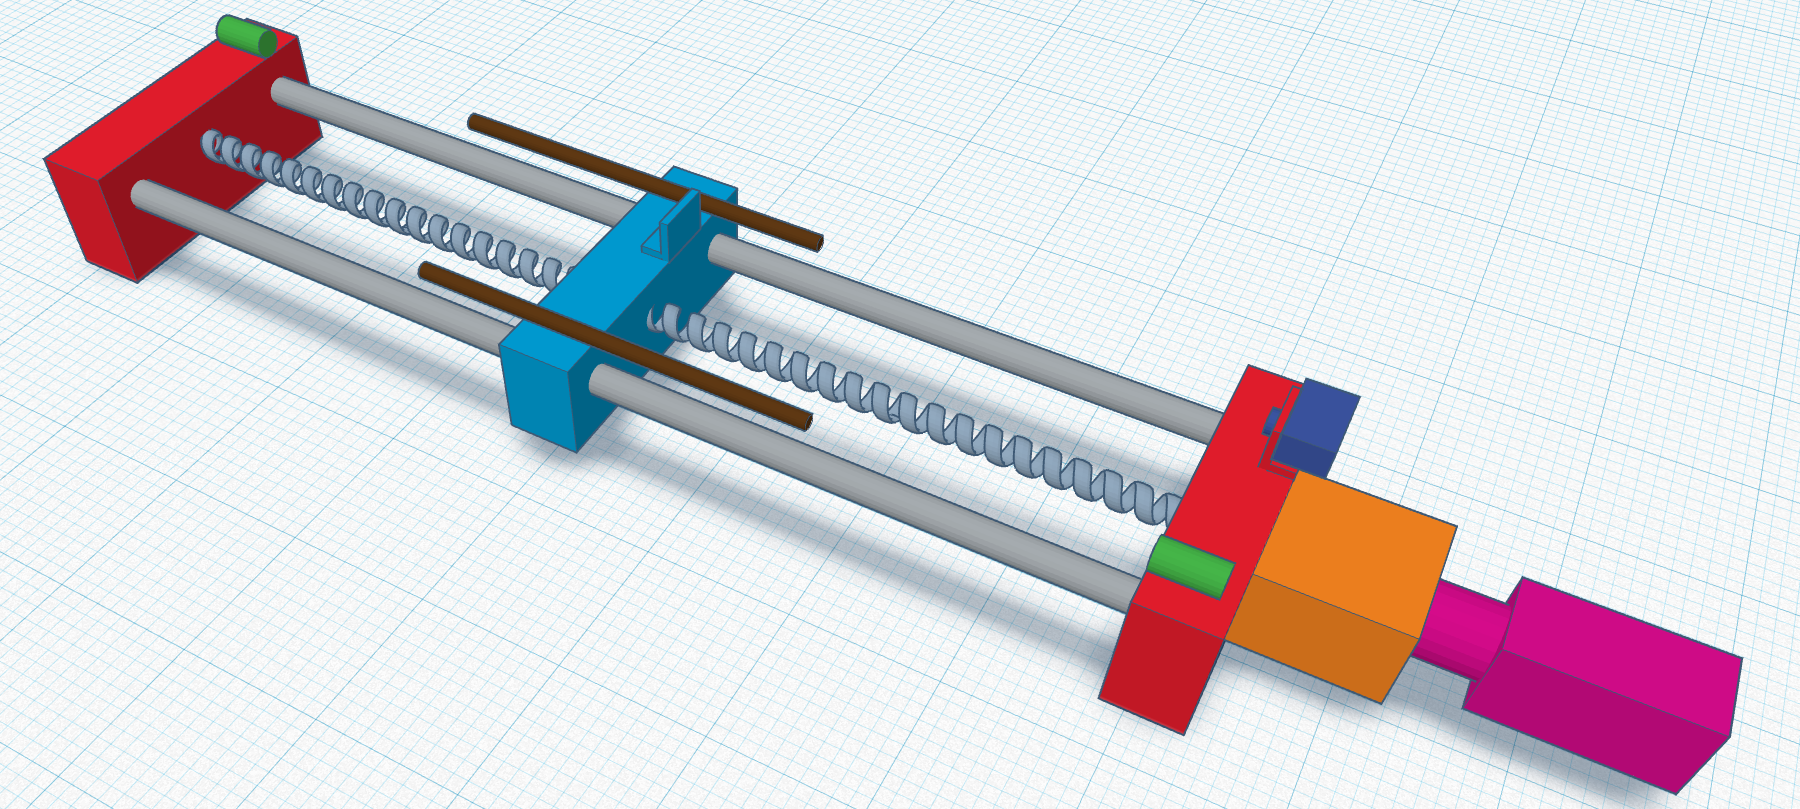
\includegraphics[width=1.0\textwidth]{images/Hardware/Linerarfuerhrung_3D_Modell.png}
	\caption{Simplifiziertes 3D Modell der Lineraführung}
	\label{fig:Systemaufbau}
\end{figure}
Da sich das Sailwind 4.0 Projekt noch in der Entwicklung befindet, existiert noch kein komplett Zusammengebauter Prototyp in dem alle Teile des Projektes zusammenfinden. Die für diese Arbeit relevante Linearführung ist bereits als eigenstehendes Objekt zusammengebaut und wie in \autoref{fig:Systemaufbau} zusehen, aufgebaut. Dabei wird die rotierende Bewegung eines BLDC Motors (Pink) mit der Hilfe eines Getriebes (Orange) und einer Gewindestange in eine Translatorische Bewegung umgewandelt, mit der der Schlitten (Hellblau) zwischen den beiden Stationären Punkten (Rot) hin und her bewegt werden kann. Die beiden Endschalter (Grün) dienen als Kollisionserkennung und können auch genutzt werden um den Bewegungsraum einzuschränken. Dabei können zwei Metallstangen (Braun) verschoben werden und geben damit vor wie viel Platz zwischen dem Schlitten und dem Stationären Elementen bleibt. Zusätzlich kann über einen Abstandssensor (dunkel Blau) die Position des Schlittens in Relation zum Abstandssensor bestimmt werden.\\

\noindent Die Linearführung soll später dazu genutzt werden um die Segel des Windkraftwerkes zu Trimmen und zu Rollen (siehe \autoref{???}). Zusätzlich zu dem präsentierten Aufbau soll sich auf dem Schlitten später ein Druckkraftsensor befinden der die Kraft auf die Rotorwelle messen soll. Dieser wurde allerdings zum Zeitpunkt der Arbeit noch nicht geliefert oder auf dem Prototypen angebracht. Getrennt vom Aufbau soll ebenfalls ein Anemometer an der Kuppel angebracht werden, das die Windrichtung und Geschwindigkeit misst.

%Hier erwähnen was Platine alles für Aufgaben hat
%Um die Segel des Windkraftwerkes jederzeit für maximale Effizienz eingestellt zu haben, müssen diese dynamisch Eingestellt werden können. Hierfür überwacht ein Controllino, die über Sensoren seine Umgebung und berechnet daraus die optimale Segel Einstellung. (KP sollte besser schon früher erwähnt werden/bzw wurde eventuell schon erwähnt)
\subsection{Ziele}
Die Hardware der Steuerung zu der eben vorgestellten Linearführung soll dabei folgende Aufgaben übernehemen:
\begin{itemize}
	\item Ansteuerung aller Sensoren und Aktoren
	\item Stromversorgung aller Komponenten
	\item Lokale Bedienung der Steuerung
	\item Ethernetkommunikation mit dem Controllino
\end{itemize}

\noindent Neben diesen Aufgaben soll die ganze Steuerung in einem zumindest Staub- und Spritzwassergeschützen Gehäuse untergebracht werden. Eine Vorgänger Gruppe hatte sich dieser Aufgabe bereits gewidmet, allerdings war der resultierende Prototyp leider nicht weiter verwendbar und hatte auch einen zu großen Formfaktor. Diese Probleme sollen in dieser Iteration ebenfalls behoben werden.

%Bei dem Entwurf der Hardware sind mehrere Dinge zu beachten. Da das Sailwind 4.0 Projekt noch in den Startschuhen steht, sind einige dieser Faktoren auch noch nicht klar Bestimmbar zum Zeitpunkt dieser Arbeit. Aus diesem Grund wurden an manchen Stellen die Design Kriterien freier oder unnötig Komplex ausgelegt.\\
%
%Um die Steuerung der Segel zu ermöglichen wird ein System benötigt das alle nötigen Akteure und Sensoren, Ansteuret und Überwacht. Hierfür soll eine Steuerelektronik Hardware entworfen werden. Da sich diese im Außeneinsatz befindet sollte diese in einem Wasserdichten Gehäuse eingeschlossen sein. Eine vorrausgehende Gruppe hatte bereits die Steuerelektronik entworfen, diese war allerdings zu groß dimensioniert und hatte einige Fehler, weswegen ebenfalls ein kleinere Formfaktor und die Behebung der Probleme als Ziel gesetzt wurden. Die Steuerelektronik soll Manuell Bedienbar sein, wewegen am Gehäuse ebenfalls eine Bedienmöglichkeit existieren sollte.

\label{Analyze_der_Aktoren_und_Sensoren}
\subsection{Analyse der bestehenden Hardware Elemente}
Um eine geeignete Steuerplatine zu entwerfen, bedarf es einer Analyse der anzusteurenden Hardware Komponenten. Diese wurden bereits von vorrausgehend Gruppen festgelegt. Diese können in die Kategorien Sensoren und Aktoren gruppiert werden. Dabei wurden die benötigte Spannung, die Stromstärke und die Schnittstellen betrachtet. Durch die Spannung und die Stromaufnahme kann später die benötigte Spurenbreite auf der Platine bestimmt werden. Die Schnittstellen geben an wie mit dem jeweiligen Gerät kommuniziert werden kann und welche davon benötigt werden.\\

\subsubsection{Sensoren}
Zu den Sensoren zählen die folgenden Komponenten:
\begin{itemize}
	\item Induktiver Endschalter: IFM IFS204
	\item Optischer Abstandssensor: IFM OGD580
	\item Anemometer: MESA WSWD
	\item Druckkraft-Sensor: Burster 8532
\end{itemize}

\noindent\textbf{Induktiver Endschalter}\newline
Zwei der IFM IFS204 Endschalter sind im Design mit eingebaut. Sie funktioneren als PNP-Schließkontakt und geben an einem Ausgang ein digitales 24V Signal aus, sobald sie ausgelöst werden. Dabei hat jeder Endschalter eine typische Stromaufnahme von <10mA und eine Betriebsspannung von 9-30V.\\

\noindent\textbf{Optischer Abstandssensor}\newline
Der Abstandssensor OGD580 funktioniert über einen Laser der vom Gerät ausgehend über eine reflektive Fläche zu diesem zurückgeworfen wird. Der Abstandsensor verfügt über ein Display das den gemessen Abstand anzeigt und über das Gerät konfigurierbar ist. Er hat eine typische Stromaufnahme von ???mA und ebenfalls eine Betriebspannung von 9-30V. Der Abstand wird über einen digitalen Ausgang, dem sog. IO-Link ausgegeben. Da dieser typischerweise nur in der Automobilbranche zum Einsatz kommt, wurde ein zusätzlicher IO-Link Konverter hinzugefügt. Der EIO104 konvertiert die digitale IO-Link Schnittstelle zu einer Analogen 4-20mA Schnittstelle mit der einfacher Umgegangen werden kann. Dabei kommt ein zusätzlicher Stromverbrauch von ???mA hinzu.\\

\noindent\textbf{Anemometer}\\
Das WSWD Anemometer wird genutzt um die Windrichtung und die Windgeschwindigkeit zu messen. Dieser basiert ebenfalls auf einer 24V Versorgungsspannung und hat je nach Konfiguration und Ausführung eine Stromaufnahme von bis zu 120mA. Er besitzt ebenfalls ein Heizelement um ihn bei sehr niedrigen Temperaturen nutzen zu können. Dieses wird allerdings im Einsatzszenario und im Prototyp nicht benötigt. Die Schnittstellen des Anenometers sind abhängig von dessen Ausführung. In der zum Einsatzkommenden Ausführung, dem WSWD1, kann neben einer Analogen Schnittstelle die Daten auch über eine Digitale RS485/RS422 Schnittstelle abgefragt werden. Die Werte können Analog entweder als ein 0/4-20/24mA Strom Signal oder als ein 0/2-8/10V Spannungs Signal ausgegeben werden. Die Digitale Schnittstelle kann neben der Datenausgabe auch zur Konfiguration des Gerätes genutzt werden und bietet eine Vielzahl an Protokollen zur Kommunikation an.\\

\noindent\textbf{Druckkraft-Sensor}\newline
Der Burster Druckkraft-Sensor war der einzige Sensor der zum Zeitpunkt der Arbeit noch nicht Bestellt wurde. Dieser wurde aber dennoch mit eingeplant. Der Druckkraft Sensor kann ebenfalls mit den typischen 24V betrieben werden und hat dabei eine Stromaufnahme von ca. 12,5mA. Die Messwerte werden hier über eine Analoge 0-10V Schnittstelle übertragen.\\
\subsubsection{Aktoren}
Zu den Aktoren zählen die folgenden Komponenten:
\begin{itemize}
	\item Gleichstrommotor: Dunkermotoren BG 45x30 SI
	\item Externe Relais
\end{itemize}

\noindent\textbf{Gleichstrommotor}\newline
Der Dunkermotor BG 45x30 SI Gleichstrommotor ist das Kernelement des Aufbaus. Da der Motor eine interne Regelung besitzt, hat er eine getrennte Leistungs- und Logikversorgung. Der Motor an sich wird dabei über den Leistungsteil bestromt, während über den Logikteil dieser gesteuert werden kann und Feedback bereitstellt. Die Betriebsspannung der Leistungs- und Logikversorgung sind 24V, wobei der Motor einen maximal zulässigen Dauerstrom von 3,8A ausgesetzt sein darf. Die Logikversorung hat eine Stromaufnahme von 100mA. Die Kommunikation mit dem Motor findet über vier Digitale- und einen Analogen Eingang statt. Der Motor stellt Feedback zum aktuellen Status über drei Ausgänge bereit. Diese geben die Drehrichtung, aktuelle Störungen und die Drehgeschwindigkeit des Motors in Impulsen an. Die Bezeichnung und Funktionen dieser Eingänge sind in \autoref{tab:digitale_Eingaenge} und \autoref{tab:andere_Ausgaenge} dargestellt.\\
% Please add the following required packages to your document preamble:
% \usepackage{graphicx}
\begin{table}[H]
	\centering
		\begin{tabular}{|c|c|c|}
			\hline
			\textbf{Eingang 1 (IN1)} & \textbf{Eingang 0 (IN0)} & \textbf{Funktion}      \\ \hline
			0                        & 0                        & Motor aus              \\ \hline
			0                        & 1                        & Linkslauf              \\ \hline
			1                        & 0                        & Rechtslauf             \\ \hline
			1                        & 1                        & Stopp mit Haltemoment  \\ \hline
			\textbf{Eingang 3 (IN3)} & \textbf{Eingang 2 (IN2)} &                        \\ \hline
			0                        & 0                        & Drehzahlvorgabe Analog \\ \hline
			0                        & 1                        & Stromvorgabe Analog    \\ \hline
			1                        & 0                        & Geschwindigkeit 1      \\ \hline
			1                        & 1                        & Geschwindigkeit 2      \\ \hline
		\end{tabular}%
	\caption{Eingänge und Funktionen des BG 45x30 SI}
	\label{tab:digitale_Eingaenge}
\end{table}
\begin{table}[H]
	\centering
	\begin{tabular}{|c|c|c|}
		\hline
		\textbf{Name} & \textbf{Wertebereich} & \textbf{Funktion}      \\ \hline
		Analog In                & 0-4092$\frac{U}{min}$                        & Drehzahlvorgabe/            \\ & 0-10V & Analogwert \\ \hline		Out 1                & 12$\frac{Impulse}{U}$                        & Aktuelle Drehzahl             \\ \hline
		Out 2                & 1 = Störung; 0 = keine Störung                        &  Fehlerangabe            \\ \hline
		Out 3              & 1 = Linkslauf; 0 = Rechtslauf                       &  Drehrichtung           \\ \hline
	\end{tabular}%
	\caption{Analoger Eingang und Digitale Ausgänge des BG 45x30 SI}
	\label{tab:andere_Ausgaenge}
\end{table}

\noindent\textbf{Externe Relais}\newline
Zum Zeitpunkt der Arbeit gab es noch keinen konkreten Verwendungszweck der zwei externen Relais, diese wurden für zusätzliche Funktionalitäten dennoch mit eingeplant und sollten über ein 24V Signal geschalten werden. Sie könnten z.B zum auslösen einer Motorbremse genutzt werden.\\

\noindent\textbf{Temperatursensor}\newline
Ähnlich zu den Relais gibt es noch keine genaueren Informationen zu einem eventuell zum Einsatz kommenden Temperatursensor. Es wurde aber dennoch ein Analoger Eingang für eine 4-20mA Schnittstelle mit eingeplant für diesen.\\

\noindent\textbf{Controllino}\newline
Der Controllino ist der zentrale Microcontroller und verwaltet alle Aktoren im System. Über diesen soll das hier zu entwerfende System, seine Befehle zur Segelausrichtung bekommen. Der Datenaustausch soll hier über Ethernet stattfinden, um die große Distanz zwischen Kuppel und Basis zu überbrücken. Zusätzlich soll die Platine von diesem ebenfalls mit Strom versogt werden.

\subsubsection{Zusammenfassung und Übersicht}
Damit sind nun alle externen anzusteurenden Komponenten abgedeckt. Die benötigte Stromversorgung sowie alle Schnittstellen sind dabei in \autoref{tab:uebersicht-externe-elemente} dargestellt. Die Verbindungen wurden ebenfalls in einem Blockschaltbild in \autoref{fig:System_Aufbau} zusammengefasst. Wobei alle blauen Pfeile die digitalen 24V Ein- und Ausgänge beschreiben.
\begin{figure}[H]
	\centering
	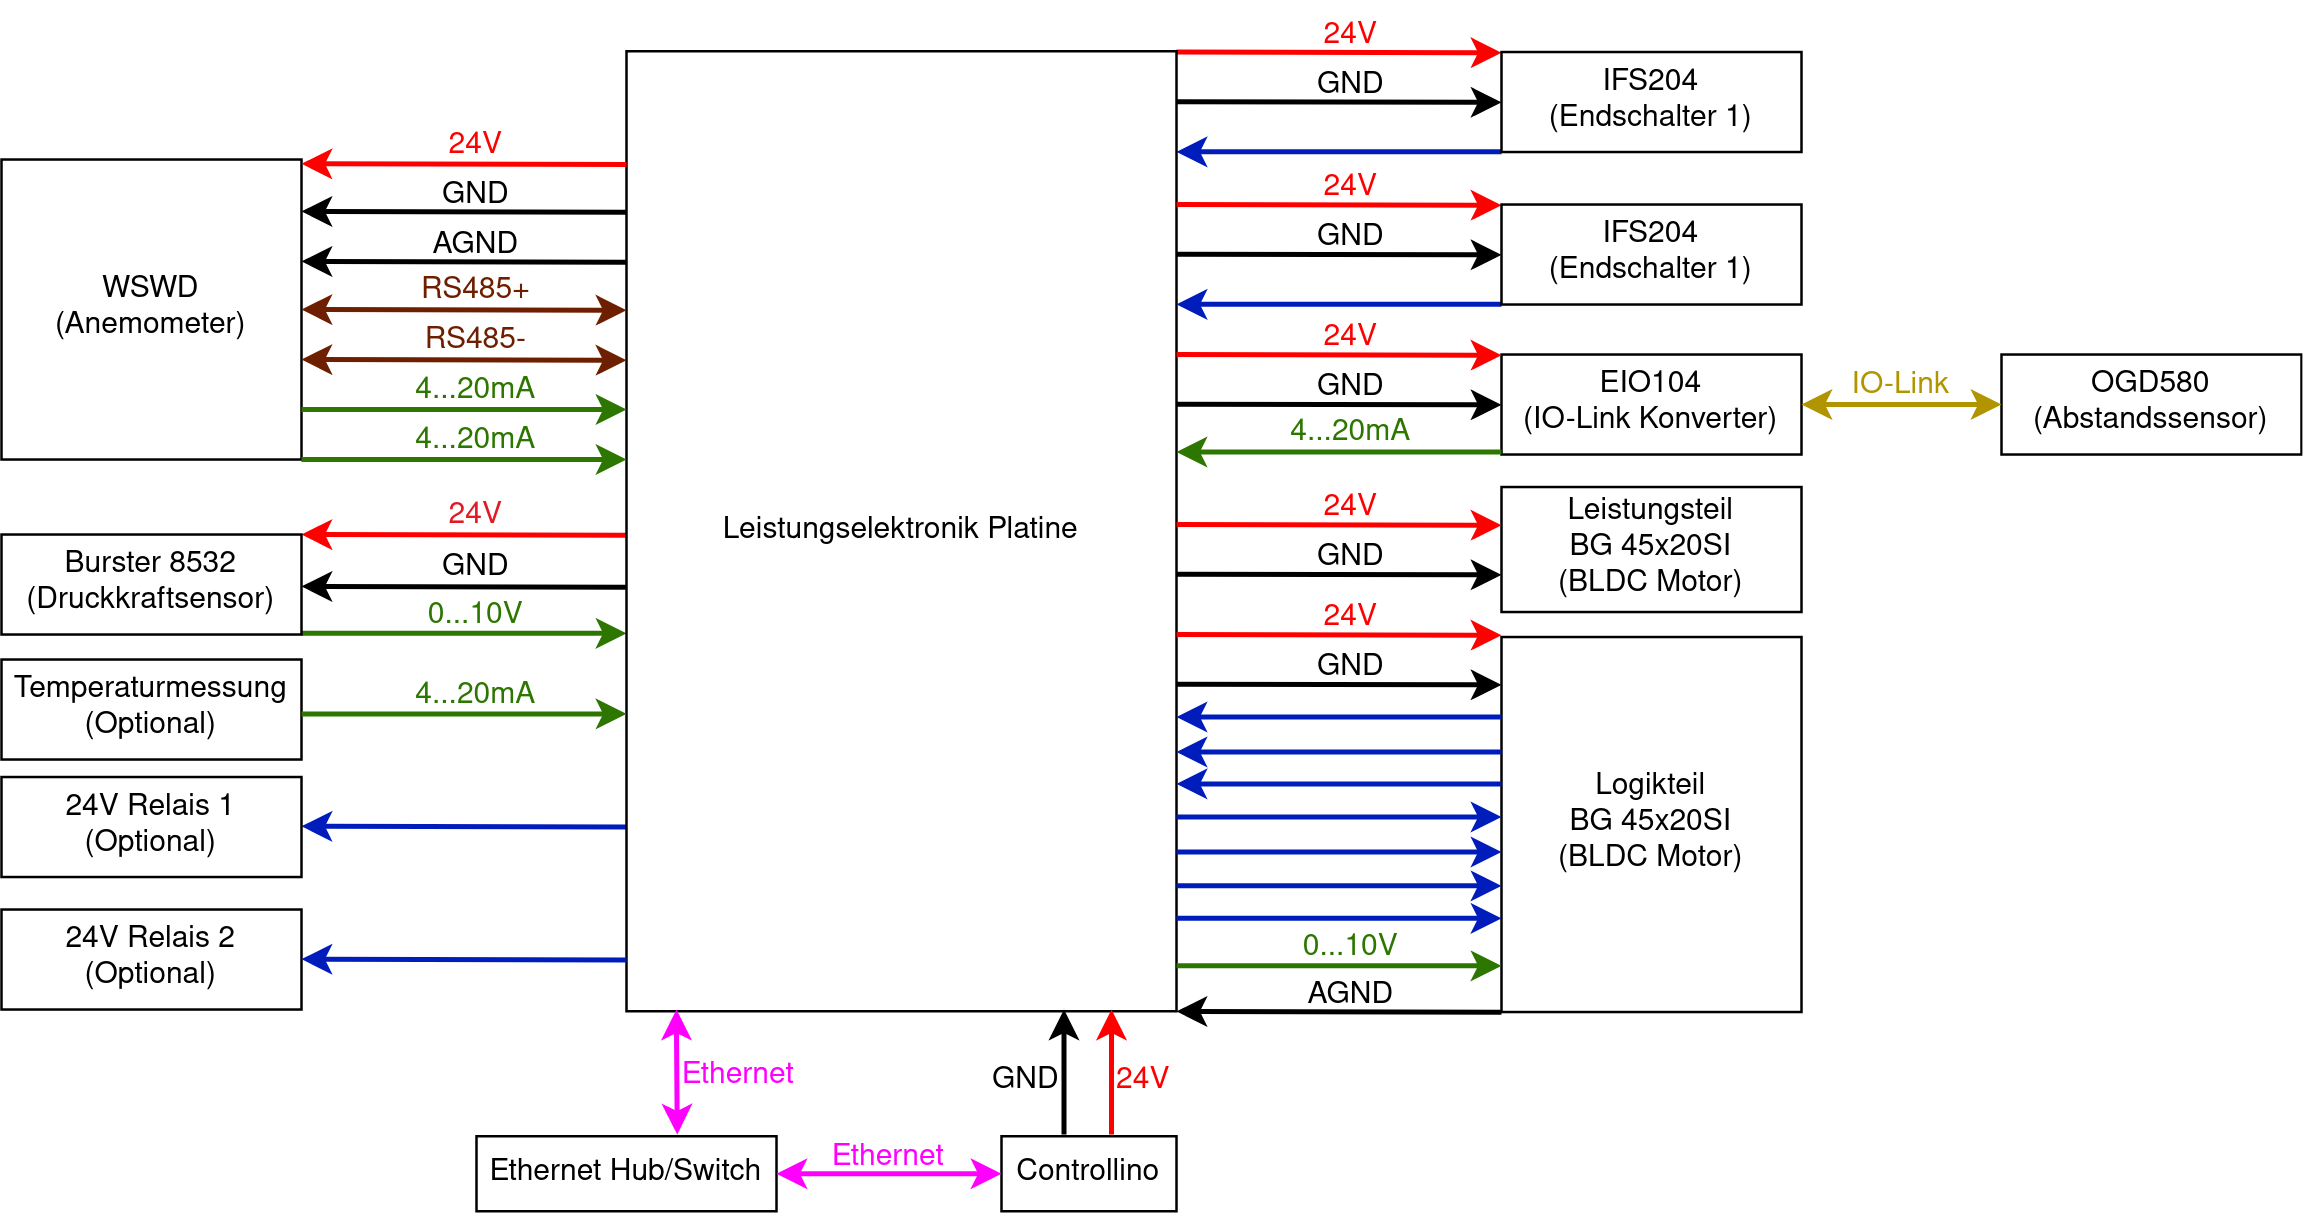
\includegraphics[width=1.0\textwidth]{images/System/Systemaufbau.drawio.png}
	\caption{Blockschaltbild der benötigten Ein- und Ausgänge der Platine}
	\label{fig:System_Aufbau}
\end{figure}
% Please add the following required packages to your document preamble:
% \usepackage{graphicx}
\begin{table}[H]
	\centering
	\resizebox{\textwidth}{!}{%
		\begin{tabular}{|l|lllllllllll|}
			\hline
			\textbf{Element} & \multicolumn{11}{l|}{\textbf{Pinout}} \\ \hline
			\textbf{Endschalter 1} & \multicolumn{1}{l|}{24V} & \multicolumn{1}{l|}{GND} & \multicolumn{1}{l|}{OUT} & \multicolumn{8}{l|}{} \\ \hline
			\textbf{Endschalter 2} & \multicolumn{1}{l|}{24V} & \multicolumn{1}{l|}{GND} & \multicolumn{1}{l|}{OUT} & \multicolumn{8}{l|}{} \\ \hline
			\textbf{Abstandssensor} & \multicolumn{1}{l|}{24V} & \multicolumn{1}{l|}{GND} & \multicolumn{1}{l|}{IO-Link} & \multicolumn{8}{l|}{} \\ \hline
			\textbf{IO-Link Konveter} & \multicolumn{1}{l|}{24V} & \multicolumn{1}{l|}{GND} & \multicolumn{1}{l|}{AOUT} & \multicolumn{8}{l|}{} \\ \hline
			\textbf{Anemometer} & \multicolumn{1}{l|}{24V} & \multicolumn{1}{l|}{GND} & \multicolumn{1}{l|}{AOUT} & \multicolumn{1}{l|}{AOUT} & \multicolumn{1}{l|}{AGND} & \multicolumn{1}{l|}{RS485+} & \multicolumn{1}{l|}{RS485-} & \multicolumn{4}{l|}{} \\ \hline
			\textbf{Druckkraftsensor} & \multicolumn{1}{l|}{24V} & \multicolumn{1}{l|}{GND} & \multicolumn{1}{l|}{AOUT} & \multicolumn{1}{l|}{AGND} & \multicolumn{7}{l|}{} \\ \hline
			\textbf{Motor Leistung} & \multicolumn{1}{l|}{24V} & \multicolumn{1}{l|}{GND} & \multicolumn{9}{l|}{} \\ \hline
			\textbf{Motor Logik} & \multicolumn{1}{l|}{24V} & \multicolumn{1}{l|}{GND} & \multicolumn{1}{l|}{IN0} & \multicolumn{1}{l|}{IN1} & \multicolumn{1}{l|}{IN2} & \multicolumn{1}{l|}{IN3} & \multicolumn{1}{l|}{AIN} & \multicolumn{1}{l|}{AGND} & \multicolumn{1}{l|}{OUT1} & \multicolumn{1}{l|}{OUT2} & OUT3 \\ \hline
			\textbf{Externes Relais 1} & \multicolumn{1}{l|}{OUT} & \multicolumn{1}{l|}{GND} & \multicolumn{9}{l|}{} \\ \hline
			\textbf{Externes Relais 2} & \multicolumn{1}{l|}{OUT} & \multicolumn{1}{l|}{GND} & \multicolumn{9}{l|}{} \\
			\hline
			\textbf{Temperatur Sensor} & \multicolumn{1}{l|}{AOUT} & \multicolumn{10}{l|}{} \\ \hline
			\textbf{Controllino} & \multicolumn{1}{l|}{Ethernet} & \multicolumn{10}{l|}{} \\ \hline
		\end{tabular}%
	}
	\caption{Übersicht Stromversorgung und Schnittstellen der externen Elemente}
	\label{tab:uebersicht-externe-elemente}
\end{table}
\subsection{Auswahl der Platinen Bauteile}
Da nun klar ist welche Anforderungen durch die anzuschließenden Geräte bestehen, kann auf Basis dieser nun weiterverfahren werden. Dabei soll im folgenden ein geeigneter Mikrocontroller, sowie die nötigen Platinenkomponenten ausgewählt werden, um mit den Sensoren und Aktoren zu kommunizieren und diese mit Strom zu versorgen.
\subsubsection{Mikrocontroller}
Die Auswahl des Mikrocontrollers wurde auf der Basis folgender Kriterien beschlossen:
\begin{itemize}
	\item Benötigte Inputs und Outputs
	\item Softwaresupport 
	\item Entwicklung
	\item Verfügbarkeit
\end{itemize}
Dabei gab es die Option den Chip als einzelnes Element direkt auf die selbst erstellte Platine einzubetten oder ein Entwicklungsboard als Basis zu nutzen und eine Erweiterungsplatine dafür zu nutzen. Es wurde sich dabei für ein Entwicklungsboard entschieden um bereits parallel zum Hardwaredesign eine geeignete Software zu entwickeln und diese bereits mit einem Prototypischen Aufbau zu testen (Vielleicht noch erwähnen, probleme bei vorheriger Gruppe). Dies bietet ebenfalls den Vorteil, das beim zerstören des Chips ein schneller Ersatz angebracht werden kann und auch bereits ein Formfaktor vorgegeben ist. Auch kann durch den bereits angebrachten Debugger, schneller neue Software getestet und aufgespielt werden. Ebenfalls besitzen viele Entwicklungsboards bereits einen Ethernetport der sowieso benötigt wird.\\

\noindent Durch die oben genannten Kriterien und die Entscheidung ein Entwicklerboard zu benutzen viel die Wahl auf das STM32 NUCLEO F439zi Board. Diese waren bereits an der HTWG Konstanz Verfügbar, sind durch den Softwaresupport von ST und ihrer eigenen Entwicklungsumgebung einfach zu Programmieren und Aufzusetzen. Außerdem bieten ihre Entwicklungsboards einen abbrechbaren Debugger und das Board kann damit auch außerhalb der Entwicklungsphase eingesetzt werden.
\subsubsection{Relais}
Um das auslösen eines Endschalters an den Mikrocontroller weiterzugeben, werden zwei 24V Relais benötigt die bei der Aktivierung der Spule ein 3,3V Signal an den Eingang des Mikrocontrollers weitergeben. Gleichzeitig soll durch die Relais der Eingang 1 oder 2 des Motors auf Null gesetzt. Diese geben die Drehrichtung an und stoppen den Motor sobald beide auf Null gesetzt sind. Da dieses System unabhängig von der Software des Mikrocontrollers agiert, sollen diese gleichzeitig als Ausfallsichere Aktoren dienen. Hierfür wurden die Omron G6S-2F 24DC Relais ausgesucht. Diese besitzen zwei Schaltbare Ausgänge und haben gleichzeitig einen kompakten Formfaktor.
\subsubsection{Optokoppler}
Um die restlichen 24V Aus- und Eingänge zu steueren oder auszulesen, kommen Optokoppler zum Einsatz. Diese isolieren ähnlich zu Relais den 24V und 3,3V Schaltkreis. Dabei werden insgesamt 9 benötigt um die digitalen Ein und Ausgänge des Motors und die beiden externen Relais zu schalten. Da es sich beim Ausgang 3? des Motors um ein Pulsierendes Signal zur Ermittelung der Drehgeschwindigkeit des Motors handelt wurde auf eine schnelle Schaltzeit der Optokoppler geachtet. Zusätzlich sollte wie bei den Relais wieder ein kleiner Formfaktor vorliegen. Hierfür wurden die LTV-817S ausgesucht. Diese haben mit einer Typischen Schaltzeit von 3-18$\mu$s eine ausreichend Schelle Schaltzeit und ihr kleiner Formfaktor lässt sie gut auf der Platine unterbringen.
\subsubsection{RS485 zu UART Konverter}
Um das Anemometer über die RS485 Schnittstelle zu konfigurieren und Daten abzufragen wird ein zusätzlicher Baustein benötigt. Dieser Konvertiert das differenzielle RS485 Signal zu einem nicht differenziellen \ac{UART} Signal, das der Mikrocontroller untertsützt. Hier wurde der MAX3485CSA+CT-ND ausgesucht da dieser mit einer 3,3V Versorgungsspannung betrieben werden kann und mit bis zu 10$\frac{MB}{s}$ Datenübertragen kann.
\subsubsection{FRAM}
Da die neutrale Position des Segels dauerhaft gespeichert werden soll, wird ein nicht flüchtiger Speicherstein benötigt. Dabei ist der \ac{FRAM} einer der billigsten Speichermöglichkeiten für diesen Zweck. Es wurde die geringste Speichergröße gewählt, da die gespeicherten Daten jederzeit, wie bei einem EEPROM Speicher, überschrieben werden könnem. Hier wurde der FM25L16B-GTR gewählt, dieser hat eine Speicher von 16Kbit und ist damit zum Speichern der Positionsdaten mehr als genügend. Da er über eine \ac{SPI} Schnittstelle angesteuert wird, sind die Schreib- und Lesegeschwindigkeiten sehr schnell. Ebenfalls ist die Lebenserwartung von 85Jahren des Speichers bei 20Mhz Taktfrquenz mehr als ausreichend.
\subsubsection{Operations Verstärker}
Um die Drehzahl des Motors vorgeben zu können, wird ein Analoges Signal im Bereich von 0-10V benötigt. Da der \ac{DAC} des Mikrocontroller bei einer Versorgungsspannung von 5V maximal ein Analoges Signal von 3,3V Ausgeben kann \cite{STM32}, wird ein Operationsverstärker benötigt. Dieser soll mit einem 24V Offset Spannung das Ausgangssignal auf bis zu 10V skalieren. Hier gab es bis auf die maximal Spannung keine großen Anforderungen an den Operationsverstärker und es wurde der weitvebreitet LM2904QS ausgewählt.
\subsubsection{DC/DC-Wandler}
Um alle Komponenten zu versorgen Bedarf es insgesamt 3 verschieden Spannungspotenzialen: 24V, 5V und 3,3V. Um dies zu erreichen sollen alle externen Komponenten direkt mit den 24V versorgt werden. Der Mikrocontroller soll mit den 5V versorgt werden, da er somit auch ohne Debugger Erweiterung genutzt werden kann \cite{STM32}. Hierfür wird ein Step Down Konverter genutzt der die 24V Versorgungsspannung auf 5V herunterbricht. Die 5V sollen daraufhin auf weitere 3,3V mit einem Festspannungsregler heruntergebrochen werden, um die sonstigen Bauteile mit dieser zu Versorgen. Bei der Auswahl wurde darauf geachtet, dass der Konverter einen ausreichenden Strom zu Verfügung stellt ohne dabei dauerhaft unter Vollast zu laufen. Da der Mikrocontroller bis zu 250mA verbraucht musste darauf geachtet werden das der Konverter mehr als diesen Strom zu Verfügung stellt. Es wurde davon Ausgegangen das die restlichen Bauteile nicht mehr als zusätzliche 250mA verbrauchen. Aus diesem Grund wurde der R-78E5.0-0.5 Ausgewählt. Dieser stell bis zu 0,5A an Strom zu Verfügung und kann bei Bedarf mit der 1A Version ausgetauscht werden. Als Festspannungsregler wurde der LM3940IMP-3.3 gewählt. Dieser kann Eingangsspannung von bis zu 7.5V in eine Ausgangsspannung von 3,3V umwandeln und hat dabei einen durchsatz Strom von bis zu 1A. Damit genügt er den Anforderungen.
\subsubsection{Strom Sensor}
Zur Überwachung des Motor Stroms kommt ein Hallstromsensor zum Einsatz. Dieser ist im Gegensatz zu einem Resistiven Sensor genauer und isoliert den 24V und 3,3V Schaltkreis. Er sollte in der Lage sein den maximal zulässigen Motorstrom messen zu können. Da die meisten Hall Sensoren deutlich mehr als diesen messen können wurde sich für den TMCS1101A3BQDRQ1 entschieden. Dieser kann einen maximalen Strom von $\pm$11,25A messen. Der gemessen Strom wird als analoges 0-3,3V Signal ausgegeben.
\subsubsection{Konnektoren}
Die externen Komponenten sollen über Schraubklemmen direkt an die Platine angeschlossen werden. Je nach Querschnitt der Kabel wurde ein größeres oder kleineres Rastermaß gewählt um Platz auf der Platine einzusparen. Dabei wurde als Standard Rastermaß 2,54mm gewählt und für die Kabel mit größerem Durchschnitt ein 3,5mm Rastermaß.
\subsubsection{Analoge Eingänge}
Um die Analogen Ausgänge des Abstandsensors und des Anemometers auszulesen wird das 4-20mA Stromsignal über einen Widerstand zu einem 0-3V Spannungssignal gewandelt das mit dem \ac{ADC} des Microcontrollers gelesen werden kann.
\subsection{Gehäusebauteile}
Um die Platine die sich später in der Kuppel befinden soll, vor z.B Staub und Wasser zu schützen soll diese in einem Gehäuse untegebracht werden. Das Gehäuse sollte vorallem im Innenraum genug Platz bieten um Kabel an der Platine zu befestigen, eine Möglichkeit bieten die Platine darin zu befestigen und genug Platz auf der Oberfläche bieten um die Bedienoberfläche und die unterschiedlichen Kabel Durchführungen zu positionieren. Dabei wurde das Hammond Manufacturing RP1465 gewählt. 
\begin{figure}[H]
	\centering
	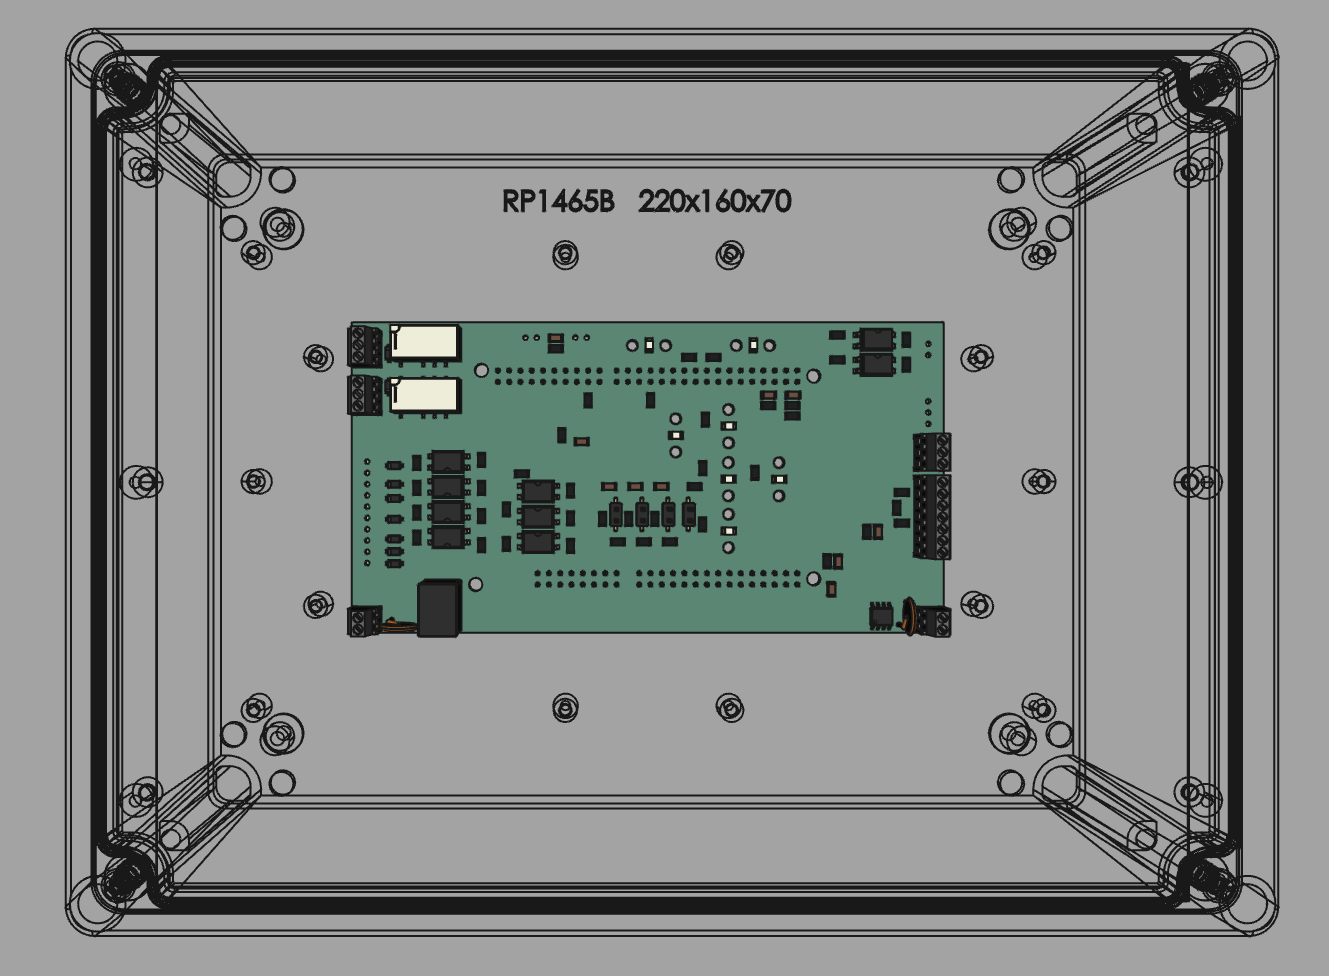
\includegraphics[width=0.8\textwidth]{images/Hardware/Platine_in_gehause.PNG}
	\caption{3D Modell der Platine innerhalb des Gehäuses}
	\label{fig:Gehaues_und_Platine}
\end{figure}
\noindent Dieses bietet genug Platz für die Platine und alle Kabeldurchführungen wie gut in \autoref{fig:Gehaues_und_Platine} zusehen ist. Es bietet ebenfalls die Möglichkeit einen zweiten Boden einzusetzen auf dem der Mikrocontroller und die Platine mit einer 3D gedruckten Befestigung angeschraubt werden können.\\

\subsubsection{Bedienoberfläche}
\noindent Die Bedienoberfläche besteht aus einer Reihe von Kippschaltern, Knöpfen und LEDs. Diese sind sind in \autoref{fig:Bedienung} dargestellt. Dabei soll die gewünschte Neutrale Position der Linearführung durch einen Kalibrierungsfahrt stattfinden. Dabei kann der Endnutzer über die Trimm und Roll Knöpfe zum gewünschten Mittelpunkt Navigieren und diesen mit dem dritten Knopf speichern. Anschließend kann mittels des Kippschalters in den Automatik Betrieb gewechselt werden in dem das betätigen der Knöpfe ignoriert wird.
Eine Reihe von LEDs gibt Feedback über den aktuellen Zustand der Linearführung. Dabei wird konstant der aktuelle Betriebsmodus durch zwei LEDs angegeben. Ebenfalls wird die Position relativ zur festgelegten neutral Position durch zwei gelbe LEDs angegeben. Eine Störung in der Steuerung oder im Motor wird durch eine rote LED angegeben.\\
Die Knöpfe und Kippschalter sind beide am Gehäuse montiert und sind durch Dichtungsringe Spritzwasser geschützt. Die Kabel werden über Dupont Stecker auf der Platine verbunden. Im Gegensatz dazu sind die LEDs direkt auf der Platine platziert und werden durch flexible Lichtleiter zur Außenseite des Gehäuses geführt.
\begin{figure}[H]
	\centering
	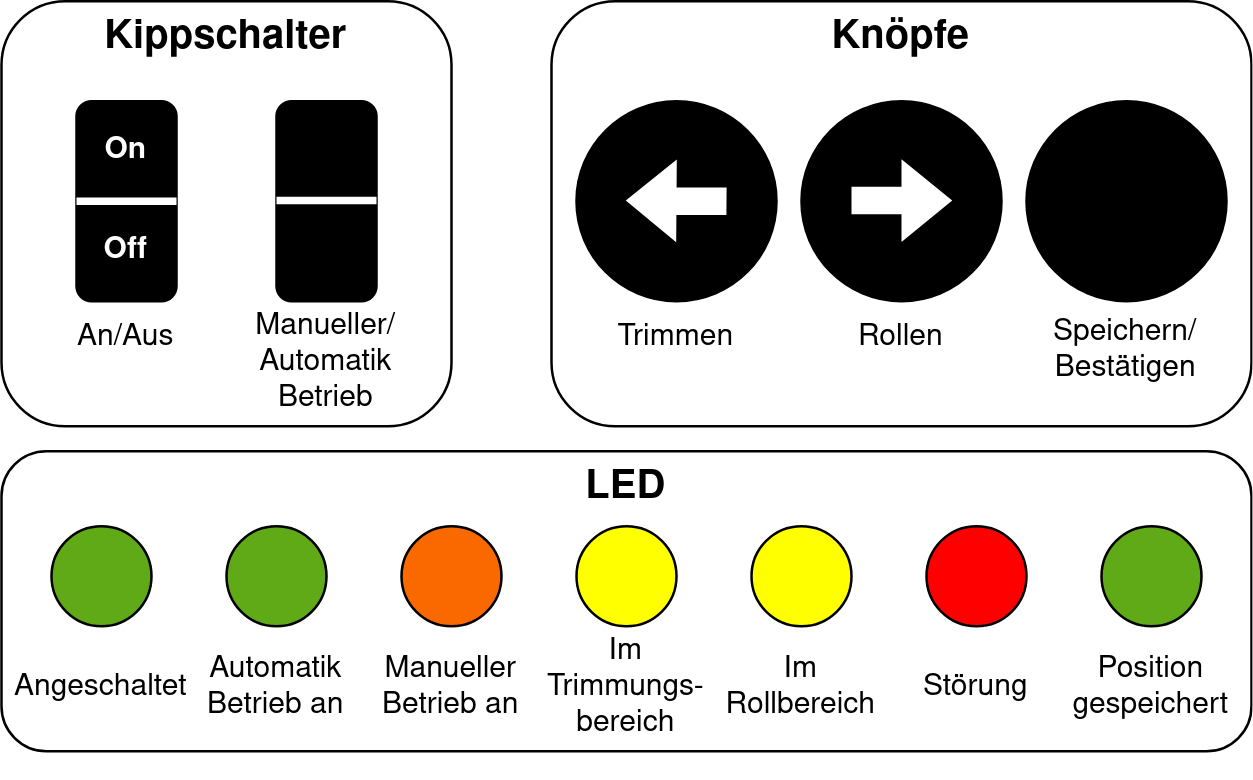
\includegraphics[width=1.0\textwidth]{images/Hardware/Bedienung.drawio.png}
	\caption{HMI der Segel Steuerung}
	\label{fig:Bedienung}
\end{figure}
\subsubsection{Kabelverschaubungen}
Um die benötigten Kabel zu Platine zu führen wurden Kabelverschraubungen in die Seiten des Gehäuses eingelassen. In diese können die Isolierten Kabel eingeführt werden und die Adernkabel an die richtige Position innerhalb des Gehäuses verlegt werden. Die Kabelverschraubungen sorgen ebenfalls für eine Zugentlastung der Kabel an sich.
\subsection{Platinen Schaltplan}
\begin{figure}[H]
	\centering
	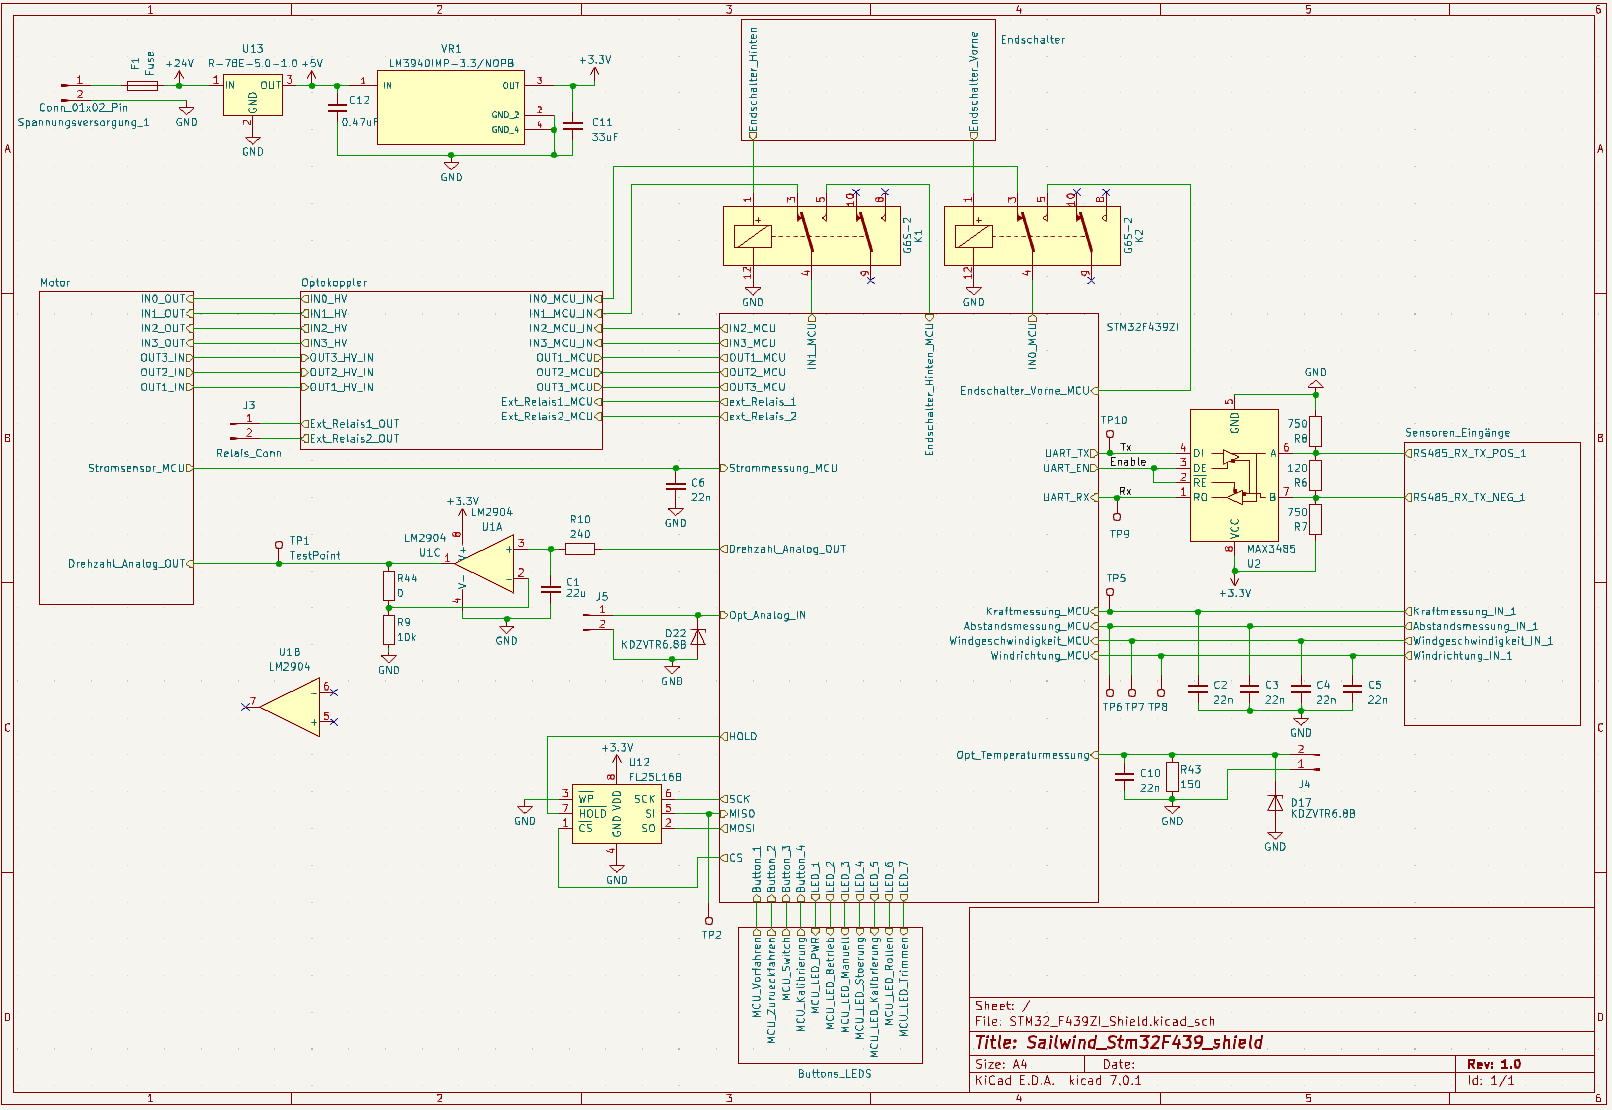
\includegraphics[width=1.0\textwidth]{images/Hardware/Schaltplan_Gesamt.PNG}
	\caption{Gesamtschaltplan der Platine}
	\label{fig:Schaltplan_gesamt}
\end{figure}
Der komplette Schaltplan ist in \autoref{fig:Schaltplan_gesamt} dargestellt und ist ebenfalls im Anhang \autoref{Anhang_Schaltplan} zu finden. Der Schaltplan ist in unterschiedliche Bereiche eingeteilt die die Gruppierung der Komponenten wiedergibt. Dabei ist die STM32 Gruppe zentral Positioniert und alle Bauteile und Komponeten um diese verteilt. Bauteile die nur einfach Verbaut sind wie z.B der FL25L16B \ac{FRAM} (Unten Links) wurden nicht in Gruppen eingeteilt sondern direkt in der Gesamtansicht Positioniert. Oben Links befindet sich die Spannungsversorgung der Platine und die \ac{DC}/DC Wandler. Überhalb des STM32 befinden sich die beiden Relais die an die Endschalter verbunden sind. Links außen befindet sich der \ac{BLDC} Motor der mit dem Operationsverstärker und den Optokoppler verbunden ist. Rechts befinden sich alle Analogen Sensoren, bis auf den Stromsensor. Dort ist ebenfalls der MAX3485 \ac{UART} Konvertierer zu sehen. Unterhalb des Mikrocontrollers befinden sich die Knöpfe und LEDS die das \ac{HMI} bilden. Im folgenden sollen exemplarisch die Schaltungen für diese Gruppen genauer betrachtet werden. Der komplette Schaltplan ist ebenfalls im Anhang hinterlegt.
\subsubsection{STM32F439zi Gruppe}
Die STM32F439zi enthält alle Pins auf denen später die Erweiterungplatine aufsitzt. Hier wurden alle benötigten Pins nach außen geführt.
\subsubsection{Motor Gruppe}
In der Motorgruppe ist neben den Ein- und Ausgängen des BG 45x30 SI auch der Hall Stromsensor abgebildet. Alle digitalen Ein- und Ausgänge auch außerhalb der Motorgruppe sind durch 24V Zener Dioden geschützt die als Überspannungsschutz agieren. Die Spannungsversorgung der Platine und des Motors sind zusätzlich durch Sicherungen vor einem Überstrom geschützt, wie anhand des Stromsensors in \autoref{fig:Motor_gruppe }zu sehen ist.
\begin{figure}[H]
	\centering
	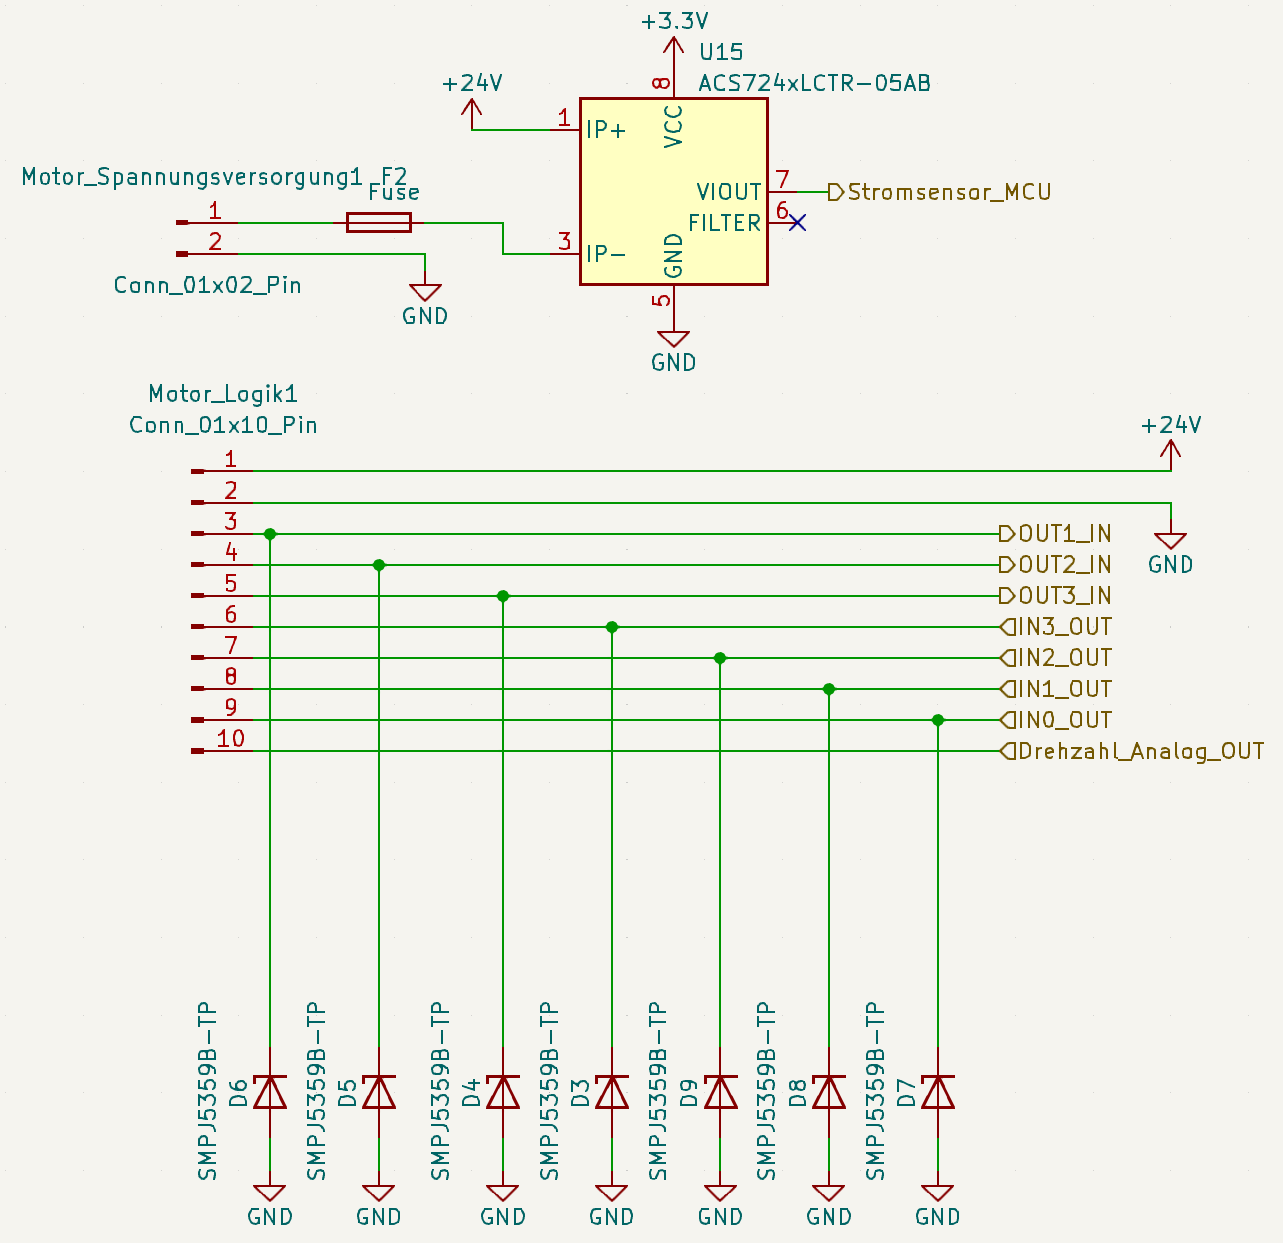
\includegraphics[width=1.0\textwidth]{images/Hardware/Motor_Schaltplan.PNG}
	\caption{Schaltplan der Motorgruppe}
	\label{fig:Motor_gruppe}
\end{figure}

\subsubsection{Optokoppler Gruppe}
\begin{figure}[H]
	\centering
	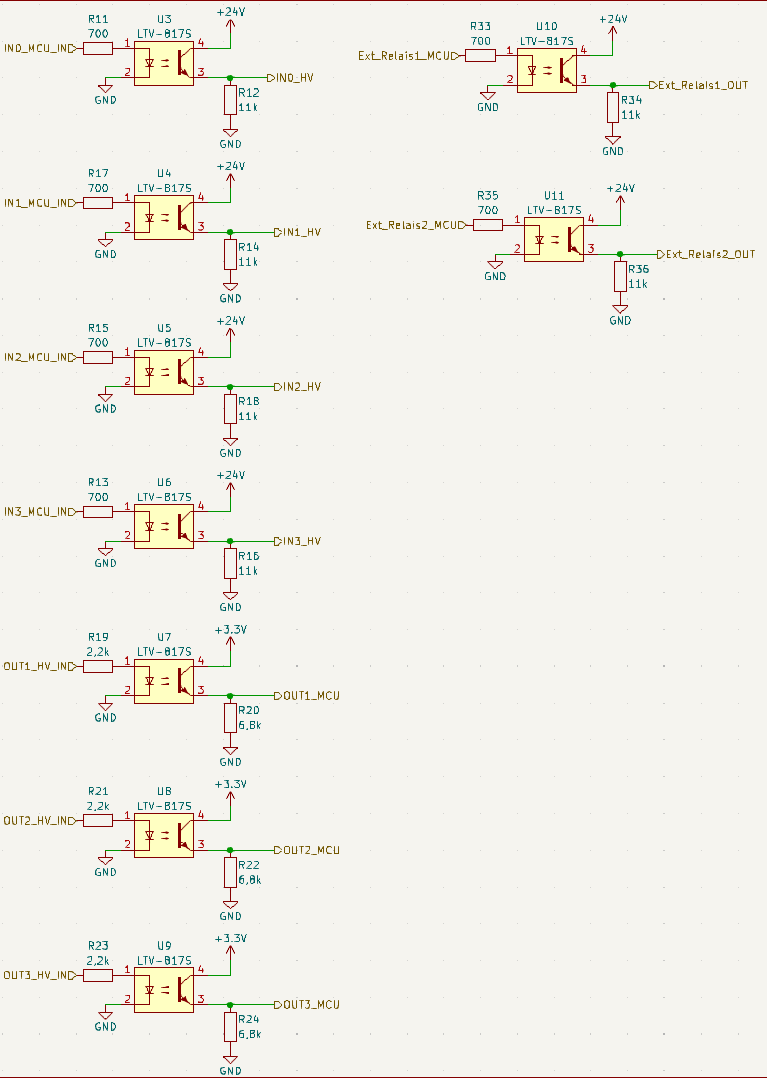
\includegraphics[width=1.0\textwidth]{images/Hardware/Optokoppler_Schaltplan.PNG}
	\caption{Schaltplan der Optokopplergruppe}
	\label{fig:Optokoppler_gruppe}
\end{figure}
Alle Optokopplerschaltungen der Gruppe sind gleich Aufgebaut. Der Eingangswiderstand (links) begrenzt den Strom der in der verbauten Infrarot LED des Optokopplers den Stromfluss auf der Ausgangsseite bestimmt. Ein Pulldown Widerstand auf der Ausgangsseite begrenzt den maximal erlaubten Strom zum Mikrocontroller und setzt den Eingang auf ein festgelegtes Potenzial.
\subsubsection{Sensoren Gruppe}
In der Sensoren Gruppe sind die Analogen Sensoren abgebildet. Hier ist gut zu erkennen wie die Strom Singale in Spannungs Signale von einem Widerstand umgewandelt werden. Für die 4-20mA Signale wurde dabei ein 150$\Omega$ Widerstand gewählt da damit bei einem maximalen Strom von 20mA fast die 3,3V erreicht werden:
\begin{equation}
	U = 20mA\times150\Omega = 3V
\end{equation}
Das Spannungssignal von dem Druckkraftsensor wird durch einen Spannungsteiler ebenfalls auf 0-3V skaliert:
\begin{equation}
	U_{Ausgang} = \frac{10V}{2300\Omega + 1000\Omega}\times1000\Omega = 3,03V
\end{equation}
Um die Analogen Signale stabiler zu halten und niedrige Frequenzen zu entfernen wurden für jedes Analoges Signal ebenfalls Keramik Puffer Kondensatoren mit einer Kapazität 22nF hinzugefügt.
\begin{figure}[H]
	\centering
	\includegraphics[width=1.0\textwidth]{images/Hardware/Sensoren_Eingänge_Schaltplan.PNG}
		\caption{Schaltplan der Buttons und LEDs}
	\label{fig:Sensoren_Gruppe}
\end{figure}
\subsubsection{Buttons und LEDs Gruppe}
Für die Buttons wurde eine Debounce Schaltung integriert, damit das Debouncing nicht über die Software geregelt werden muss. Hierbei wurde ein RC Filter genutzt. Beim drücken des Knopfes wird der Kondensator dabei zuerst entladen was zu einer langsam abfallend Spannung führt. Wird der Knopf losgelassen lädt sich dieser wieder auf. Somit kommt nie ein Sprung innerhalb der Spannung vor. Da die Debounce Zeit der Knöpfe typisch bei 0,1ms liegt wurde von einer Zeitkonstante $\tau$ = 10ms für den RC Filter ausgegangen. Die \ac{LED}s wurden je nach zulässigen Strom mit einem entsprechenden Widerstand versehen.
\begin{figure}[H]
	\centering
	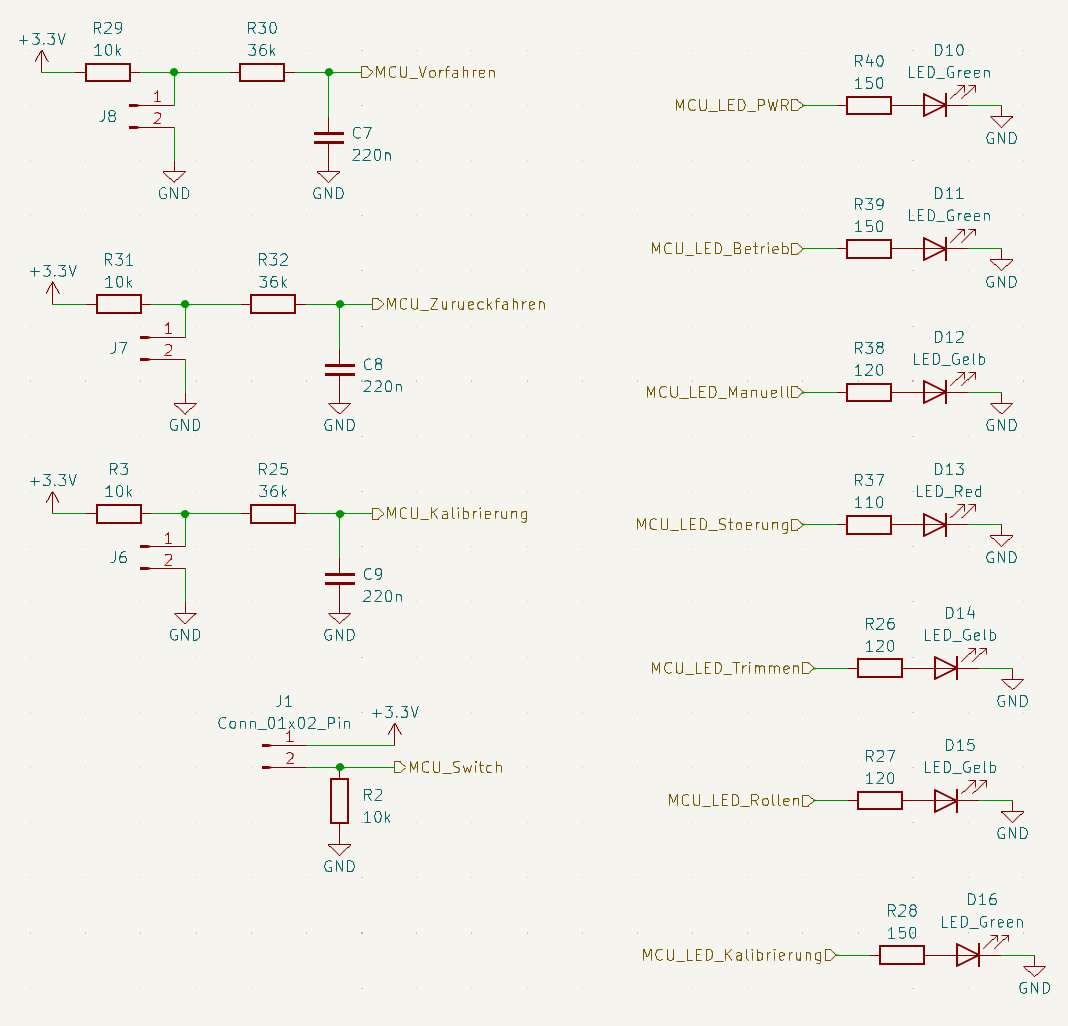
\includegraphics[width=1.0\textwidth]{images/Hardware/LEDS_und_buttons_schaltplan.PNG}
	\caption{Schaltplan der Buttons und LEDs}
	\label{fig:HMI_Gruppe}
\end{figure}
\subsection{\ac{PCB}}
Das fertige PCB ist als 3D Modell in \autoref{fig:PCB_3D} dargestellt. Beim Positionieren der Komponenten wurde daraufgeachtet die 24V Komponenten von den 3,3V Komponenten zu trennen. Aus diesem Grund befinden sich die 24V Komponenten am Rand der Platine während die 3,3V Bauteile mehr im inneren der Platine Positioniert sind. Die Platine sitzt mit vier unterschiedlichen Pin Reihen auf dem Entwicklungsboard auf und führt die Pins auf die Oberseite der Platine. Die dicke der Spuren auf der Platine wurde durch den Strom, die Spannung und Länge bestimmt. Da der Hersteller der Platine vorgegeben hat, das die kleinste Spurbreite 0,2mm sein kann, reichte diese für die meisten Spuren aus. Die Spur über die der Motorstrom fließt ist dabei die einzige breitere, da diese bis zu ca. 4A standhalten muss.
\begin{figure}[H]
	\centering
	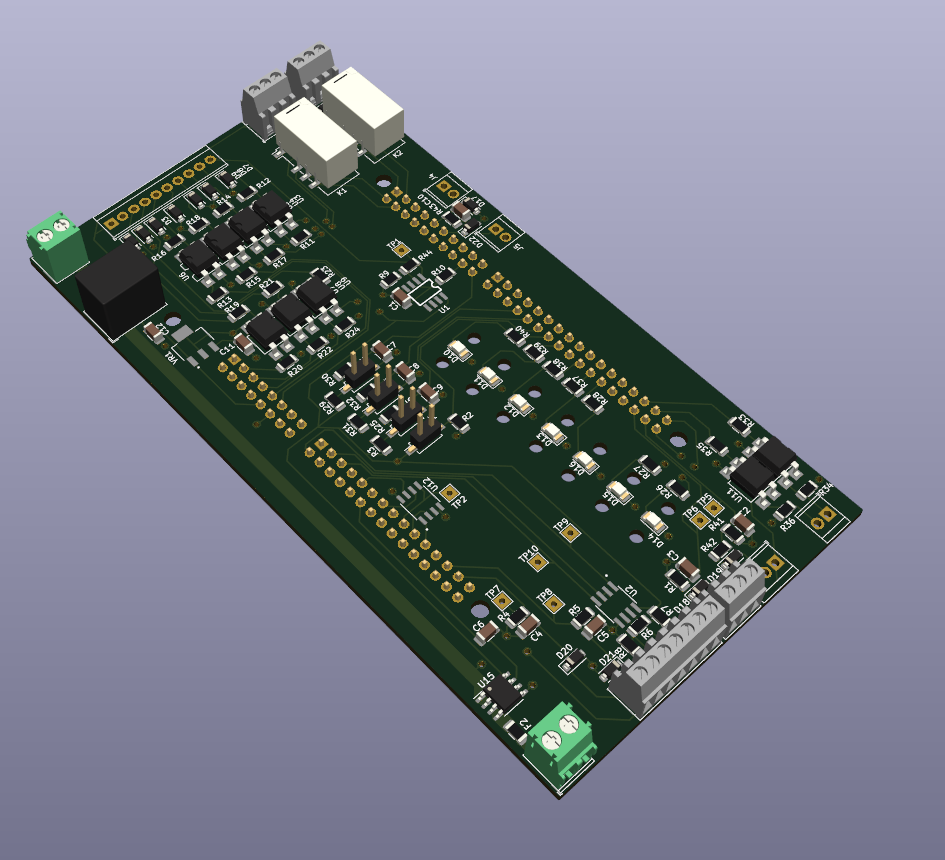
\includegraphics[width=1.0\textwidth]{images/Hardware/Platine_Fertig_3D_ansicht(1).PNG}
	\caption{3D Ansicht des fertigen PCBs}
	\label{fig:PCB_3D}
\end{figure}


\subsection{Probleme}
Während der Nutzung und Bestückung des \ac{PCB}s sind einige Probleme aufgetreten. Diese waren auf das Design oder falsche Berechnungen zurückzuführen. Diese sollen im folgenden erklärt und korrigiert werden.
\subsubsection{Schraubklemmen Löcher}
Der erste Fehler der zu Beginn auffiel, war der Durchmesser der Löcher für die Schraubklemmen. Diese waren zwar groß genug dimensioniert um die Pins Schraubklemmen durchzuführen, aber waren nicht darauf angepasst Nieten einzufügen um die Pins elektrisch mit der Platine zu verbinden. Die Löcher waren ebenfalls zu klein um mit Drähten eine elektrische Verbindung zwischen dem Pin und dem Board herzustellen. Dies führte zu vielen elektrischen Kontakt Problemen und minderte die horizontale Stabilität der Schraubklemmen. Die Kontakt Probleme führten auch zur mangelnden Präzision der Analog Eingänge (siehe \autoref{Mangelnde_Präzision}).
\subsubsection{Operationsverstärker}
Der Operationsverstärker war zwar als Verstärkerschaltung richtig konfiguriert, allerdings musste die Verstärkerspannung von 3,3V auf 24V angehoben werden, um die 10V zu erreichen. Zusätzlich wurde der Spannungsteiler am Ausgang des OPVs entfernt und der erste Widerstand gegen einen 0Ohm Widerstand getauscht.
\subsubsection{RS485 Bias Widerstände}
Die RS485 Widerstände wurden anfänglich die empfohlenen Widerstände in der WSWD Dokumentation genutzt. Hier wurde bei einer Versorgungsspannung von 5V ein Busabschlusswiderstand $R_t$ von 120$\Omega$ und zwei Biaswiderstände $R_b$ von 750$\Omega$ empfohlen (vgl.\cite{WSWD} S.21). Dies sorgte allerdings für eine zu große Differenz der beiden Spannungen und der MAX3485 konnte nicht zwischen high und low unterscheiden. Deshalb wurde stattdessen nach der Anleitung des MAX3485 die Differenz zwischen beiden Potenzialen auf 0,2V begrenzt. Hierfür wurde auf die Berechnung in dem von Texas Instruments veröffentlichten Bericht: \glqq{}RS-485 failsafe for an idle bus\grqq{} zurückgegriffen. Hier lässt sich anhand der Formel: 
\begin{equation}
	R_b = (\frac{V_s}{V_{diff }}+1)\times27,8\Omega
\end{equation}
die beiden Bias Widerstände für das RS-485 Netzwerk berechnen. Dabei kam für die Eingesetzten Werte:
\begin{equation}
	R_b = (\frac{3,3V}{0,2V}+1)\times27,8\Omega = 486,5\Omega
\end{equation}
Der nächst kleinere Widerstand der Verfügbaren E24 Reihe wurde dann auf 470$\Omega$ gewählt. Damit konnte daraufhin erfolgreich über RS485 kommuniziert werden.
\subsubsection{FRAM Anschlüsse}
Die SPI Anschlüsse des FRAM Speicher wurden falsch verbunden dabei wurden die \ac{MOSI} und \ac{MISO} Leitung vertauscht und der \ac{WP} Pin auf das Ground Potenzial gelegt. Dies führte dazu, dass der Speicher nicht addressiert werden konnte und er nicht auf gesendete Befehle reagiert hat. Zuerst wurde der \ac{WP} von dem Ground Potenzial entfernt und schwebend gehalten. Durch das Beobachten der Pegel von MISO, MOSI und Clock Leitung konnte daraufhin erkannt werden das diese vertauscht wurden. Die PCB Spur wurde dafür getrennt und die Pins mit Kabeln direkt verbunden.
\subsubsection{Abstandssensor Präzision}
Der Abstandssensor war eine weitere große Problem Quelle. Der Abstandsensor hat eine sehr hohe Präzision erreicht diese allerdings erst nach einer Aufwärmzeit. Diese ist laut Datenblatt erst bei einer Umgebungstemperatur von -10°C notwendig (vgl. \cite{OGD580_Datasheet} S.2). Allerdings wurde im Betrieb festgestellt das bei stillstand das Display des Sensors immer sinkende Werte anzeigt. Um die Ursache dafür zu finden wurden einige Messreihen durchgeführt. Hierbei wurde der Abstand zum Sensor konstant gehalten und in einem Interval von 30s der Spannungswert an einem Messpunkt der Platine mit einem Oszilloskop gemessen. Dies wurde für inkrementierende Außerbetriebszeiten wiederholt. Die Messreihe ist in \autoref{OGD580} dargestellt. Hier ist klar erkennbar das erst nach ca. 1400s oder ca 20-25min. ein gleichbleibender Spannungswert auslesbar ist. Ebenfalls geht hier hervor, dass die Präzision mit der Temperatur des Sensors zusammenhängt, da nach kürzeren Außerbetriebszeiten die Differenz sinkt.
\begin{figure}[H]
	\centering
	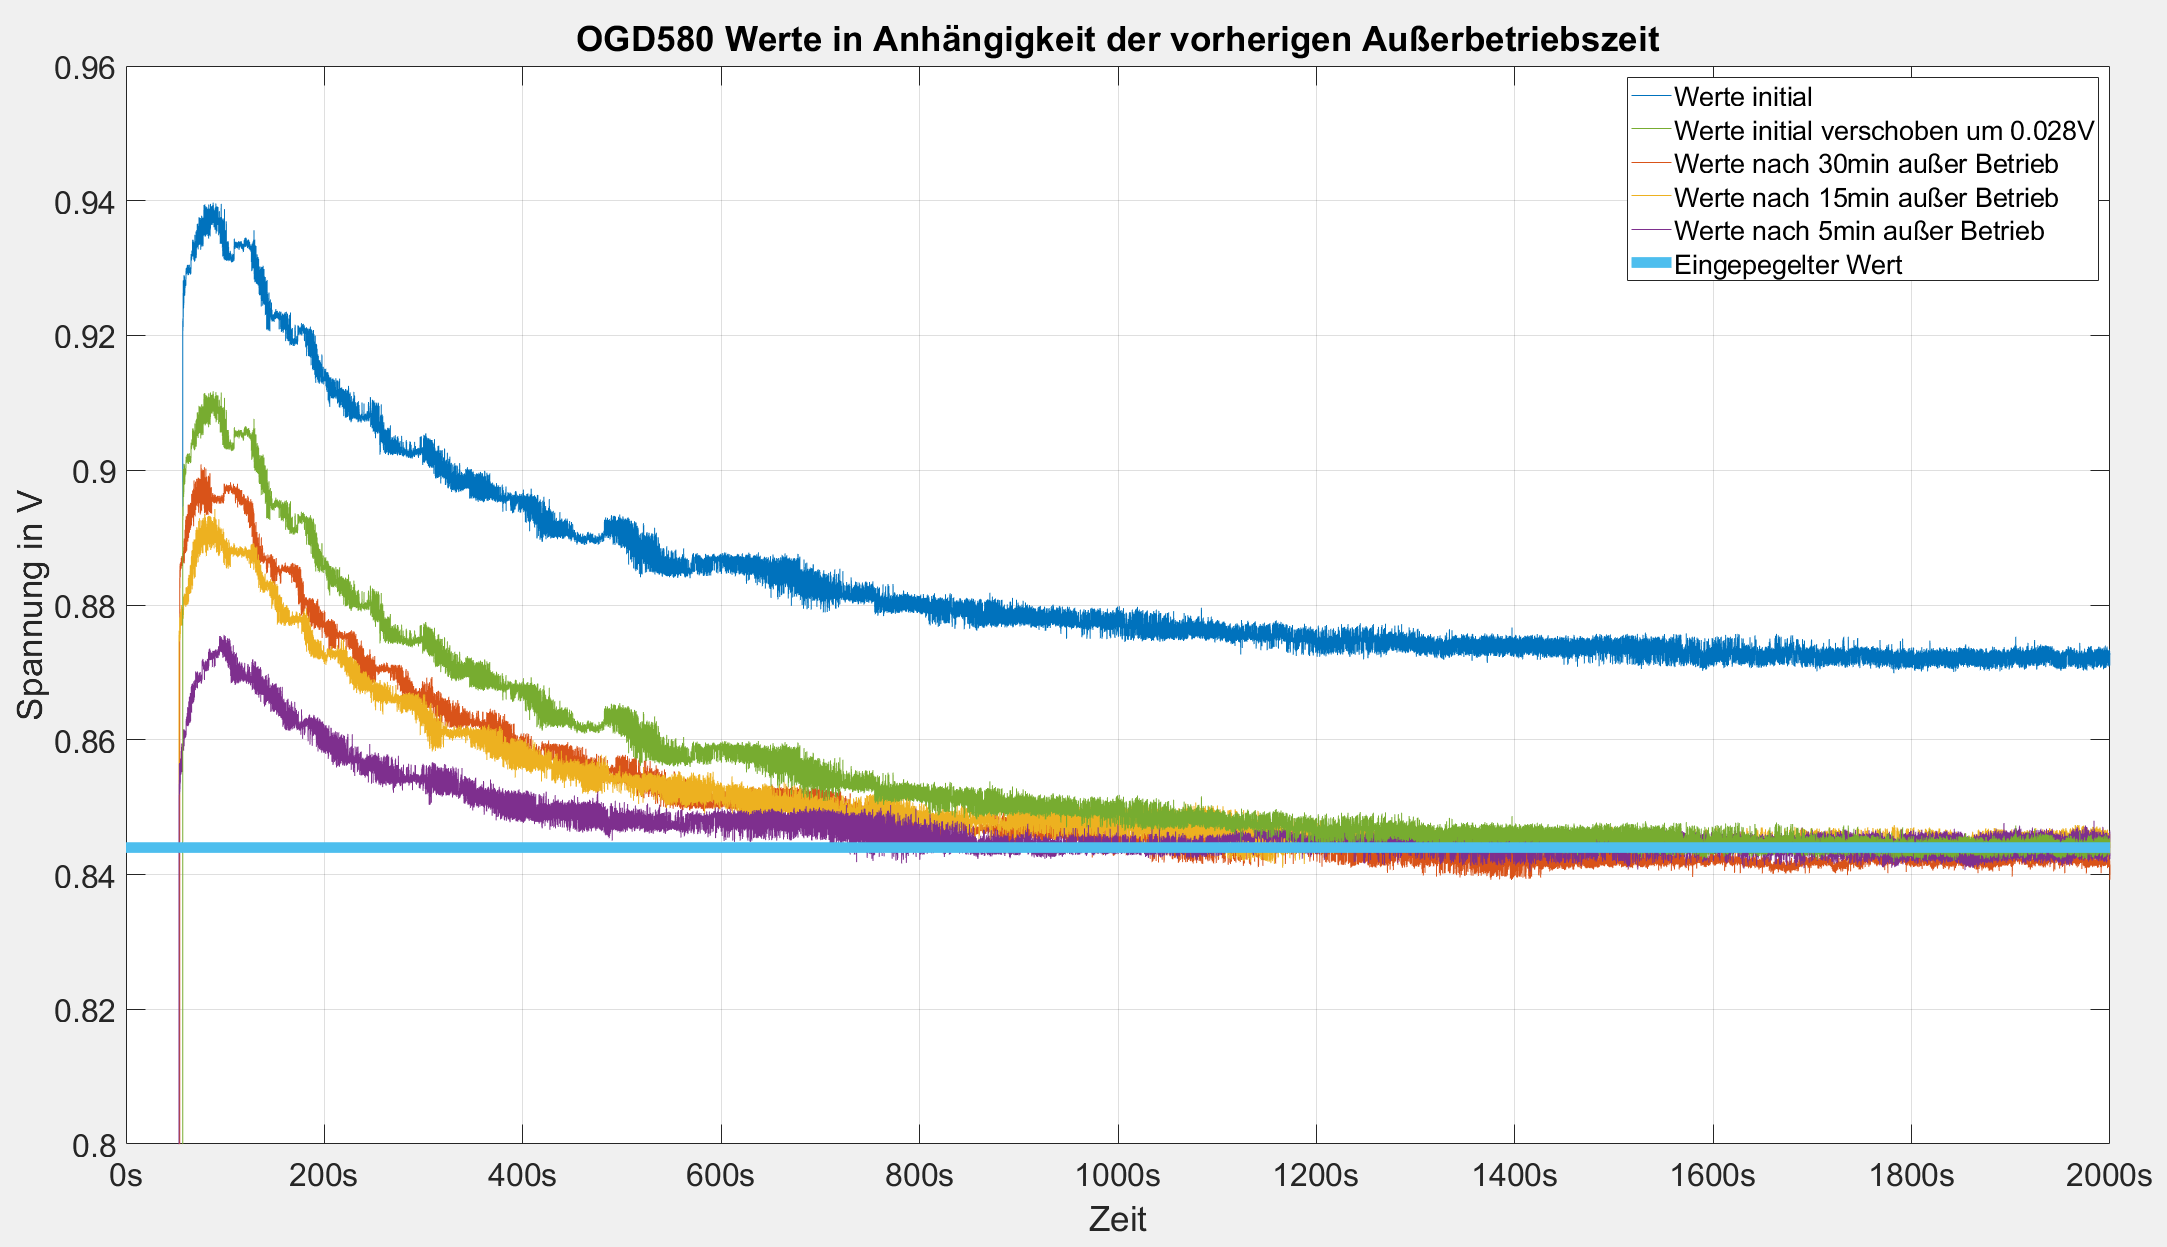
\includegraphics[width=1.0\textwidth]{images/Hardware/Abstandssensor_plot_highres.PNG}
	\caption{Messreihen des ausgelesen Spannungswert bei gleichbleibendem Abstand und steigenden Außerbetriebszeiten}
	\label{fig:Messreihe_Temperatur}
\end{figure}

Das Problem blieb allerdings selbst nach einer Aufwärmzeit von 20min. bestehen. Die Abweichung der ausgelesen Werte über die Messpunkte und den abgelesen Wert am Display lagen teilweise bis zu 25mm auseinander. Um die Ursache des Problems zu finden wurde hier ebenfalls mehrere Messreihen aufgenommen. Hier wurde der Schlitten der Linearführung in 20mm Abständen verschoben. An jedem dieser Punkte wurden folgende Daten notiert:
\begin{itemize}
	\item Abstand zum Sensor gemessen mit einem Meterstab in mm
	\item Angezeigter Abstand auf dem Display des Sensors in mm
	\item Ausgegebener Strom des IO-Link Konverters gemessen mit einem Multimeter in mA
	\item Spannung am Testpunkt der Platine mit einem Oszilloskop in V
\end{itemize}
Dies wurde in 5 Messreihen wiederholt um die Reproduzierbarkeit zu verifizieren. Die aufgezeichneten Daten wurden alle in mm umgerechnet:
\begin{equation}
	L_{Strom} = \frac{L_{max}-L_{min}}{I_{max}-I_{min}}\times(\frac{I_{Position}}{1000}-I_{min}) + L_{min}
\end{equation}
\begin{equation}
	L_{Spannung} = \frac{L_{max}-L_{min}}{I_{max}-I_{min}}\times(\frac{U_{Position}}{153,5\Omega}-I_{min}) + L_{min}
\end{equation}
 und überhalb der mit dem Meterstab gemessen Werte geplotet. Eine dieser Messreihen ist in \autoref{fig:Messreihe_Abstand} dargestellt.
\begin{figure}[H]
	\centering
	\includegraphics[width=1.0\textwidth]{images/Hardware/Messreihe_Präzision.png}
	\caption{Präzision des Abstandssensor anhand verschiedener Messwerte}
	\label{fig:Messreihe_Abstand}
\end{figure}
\noindent Hier ist zu erkennen das der auf dem Display abgelese Abstand mit dem gemessenen Abstand übereinstimmt. Allerdings weichen sowohl der Strom als auch der Spannungswert ab, da die Steigung beider Messreihen nicht gleich zu der des Abstandssensor ist. An diesem ist es möglich eine Skalierung festzulgen. Dabei kann z.B festgelegt werden ab welchem Messwert das Ausgangssignal 4mA/20mA beantragen soll (vgl. \cite{EIO104_Manual}, S.6). Da das Display den korrekten Wert anzeigt, aber ein falscher Strom Wert ausgegeben wird kann davon ausgegangen werden das der Konverter falsch eingestellt ist. Dies konnte im Zuge dieser Arbeit nicht behoben werden, da ein entsprechendes IO-Link Master Gerät nicht verfügbar war.
\subsubsection{Präzision der Analogen Signale}
Neben den Problemen mit den Abstandssensor wurden ebenfalls leicht abweichende Werte in den anderen Analog Signalen festgestellt. Beginnend mit den Strom Signalen, kann der ausgelesene Wert mit der Präzision des Widerstandes zusammenhängen, da diese mit 1\% Genauigkeit immer noch große Temperaturabweichungen aufweisen können. Die schlechten Kontakte tragen ebenfalls zur Ungenauigkeit bei. Speziell bei dem Stromsensor kann es sich ebenfalls um ein positionierungs Problem handeln, da die Verbunden Spuren für optimale Präzision im 45° Winkel zu den Sensor Pins stehen sollten. Um Präzision zu verbessern sollten zusätzlich zu den Präzisieren Widerstände ebenfalls Ferrite eingesetzt werden. Diese verhalten sich ähnlich wie Spulen und filtern hoch Frequente Signale. In Kombination mit den bereits genutzen Kondensatoren sollten diese als LC-Filter funktionieren und einen Bandpass erzeugen.\\
Bilder
